% Preamble: \usepackage{tikz}. Each version scales to its maximum measured workflow duration; compare ms values across versions.
\begin{figure}[htbp]
\centering
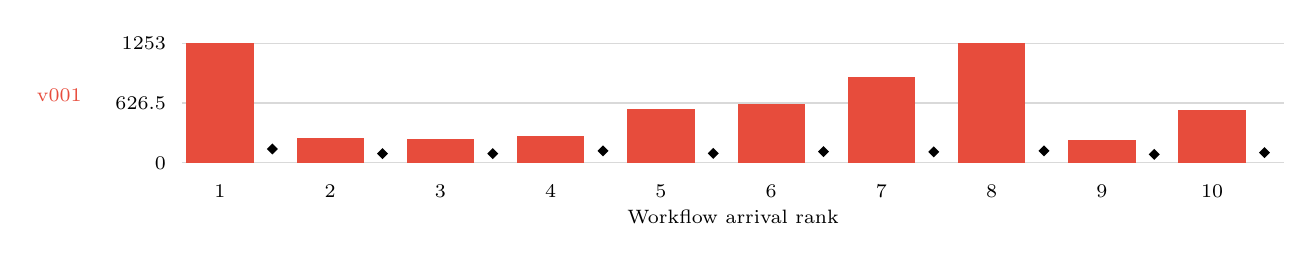
\begin{tikzpicture}[x=1.40000cm,y=1.9cm,font=\scriptsize]
\definecolor{lane0}{RGB}{231,76,60}
\node[anchor=east,text=lane0] at ([xshift=-1.15cm]0,0.450) {v001};
\draw[gray!30] (0,0.000)--(10,0.000);
\node[anchor=east] at ([xshift=-0.08cm]0,0.000) {0};
\draw[gray!30] (0,0.400)--(10,0.400);
\node[anchor=east] at ([xshift=-0.08cm]0,0.400) {626.5};
\draw[gray!30] (0,0.800)--(10,0.800);
\node[anchor=east] at ([xshift=-0.08cm]0,0.800) {1253};
\filldraw[fill=lane0,draw=lane0] (0.045,0.000) rectangle (0.645,0.796);
\fill[black] (0.7700,0.0926)--(0.8200,0.1294)--(0.8700,0.0926)--(0.8200,0.0557)--cycle;
\filldraw[fill=lane0,draw=lane0] (1.045,0.000) rectangle (1.645,0.160);
\fill[black] (1.7700,0.0613)--(1.8200,0.0981)--(1.8700,0.0613)--(1.8200,0.0245)--cycle;
\filldraw[fill=lane0,draw=lane0] (2.045,0.000) rectangle (2.645,0.158);
\fill[black] (2.7700,0.0613)--(2.8200,0.0981)--(2.8700,0.0613)--(2.8200,0.0245)--cycle;
\filldraw[fill=lane0,draw=lane0] (3.045,0.000) rectangle (3.645,0.174);
\fill[black] (3.7700,0.0798)--(3.8200,0.1167)--(3.8700,0.0798)--(3.8200,0.0430)--cycle;
\filldraw[fill=lane0,draw=lane0] (4.045,0.000) rectangle (4.645,0.356);
\fill[black] (4.7700,0.0632)--(4.8200,0.1001)--(4.8700,0.0632)--(4.8200,0.0264)--cycle;
\filldraw[fill=lane0,draw=lane0] (5.045,0.000) rectangle (5.645,0.389);
\fill[black] (5.7700,0.0753)--(5.8200,0.1122)--(5.8700,0.0753)--(5.8200,0.0385)--cycle;
\filldraw[fill=lane0,draw=lane0] (6.045,0.000) rectangle (6.645,0.567);
\fill[black] (6.7700,0.0734)--(6.8200,0.1103)--(6.8700,0.0734)--(6.8200,0.0366)--cycle;
\filldraw[fill=lane0,draw=lane0] (7.045,0.000) rectangle (7.645,0.800);
\fill[black] (7.7700,0.0804)--(7.8200,0.1173)--(7.8700,0.0804)--(7.8200,0.0436)--cycle;
\filldraw[fill=lane0,draw=lane0] (8.045,0.000) rectangle (8.645,0.147);
\fill[black] (8.7700,0.0562)--(8.8200,0.0930)--(8.8700,0.0562)--(8.8200,0.0193)--cycle;
\filldraw[fill=lane0,draw=lane0] (9.045,0.000) rectangle (9.645,0.349);
\fill[black] (9.7700,0.0677)--(9.8200,0.1045)--(9.8700,0.0677)--(9.8200,0.0308)--cycle;
\node[below] at (0.345,-0.08) {1};
\node[below] at (1.345,-0.08) {2};
\node[below] at (2.345,-0.08) {3};
\node[below] at (3.345,-0.08) {4};
\node[below] at (4.345,-0.08) {5};
\node[below] at (5.345,-0.08) {6};
\node[below] at (6.345,-0.08) {7};
\node[below] at (7.345,-0.08) {8};
\node[below] at (8.345,-0.08) {9};
\node[below] at (9.345,-0.08) {10};
\node[below] at (5.000,-0.25) {Workflow arrival rank};
\end{tikzpicture}
\caption{Processes: v001: petrinet/Workflow/P1\_Tutorial\_Workflow. Bars show measured workflow elapsed time; diamonds show maximum observed service-visit queue wait, including fork branches. Queue markers do not represent total workflow waiting time. Each version scales to its maximum measured workflow duration; compare ms values across versions. Showing 10 of 10 observed root workflows. Fork children contribute to their family's queue maximum. All shown workflows have measured elapsed and queue values. Arrival order uses GENERATED timestamps, or recorded starts for legacy rows.}
\label{fig:workflow-elapsed-queue}
\end{figure}
